\loesung{
\begin{center}
	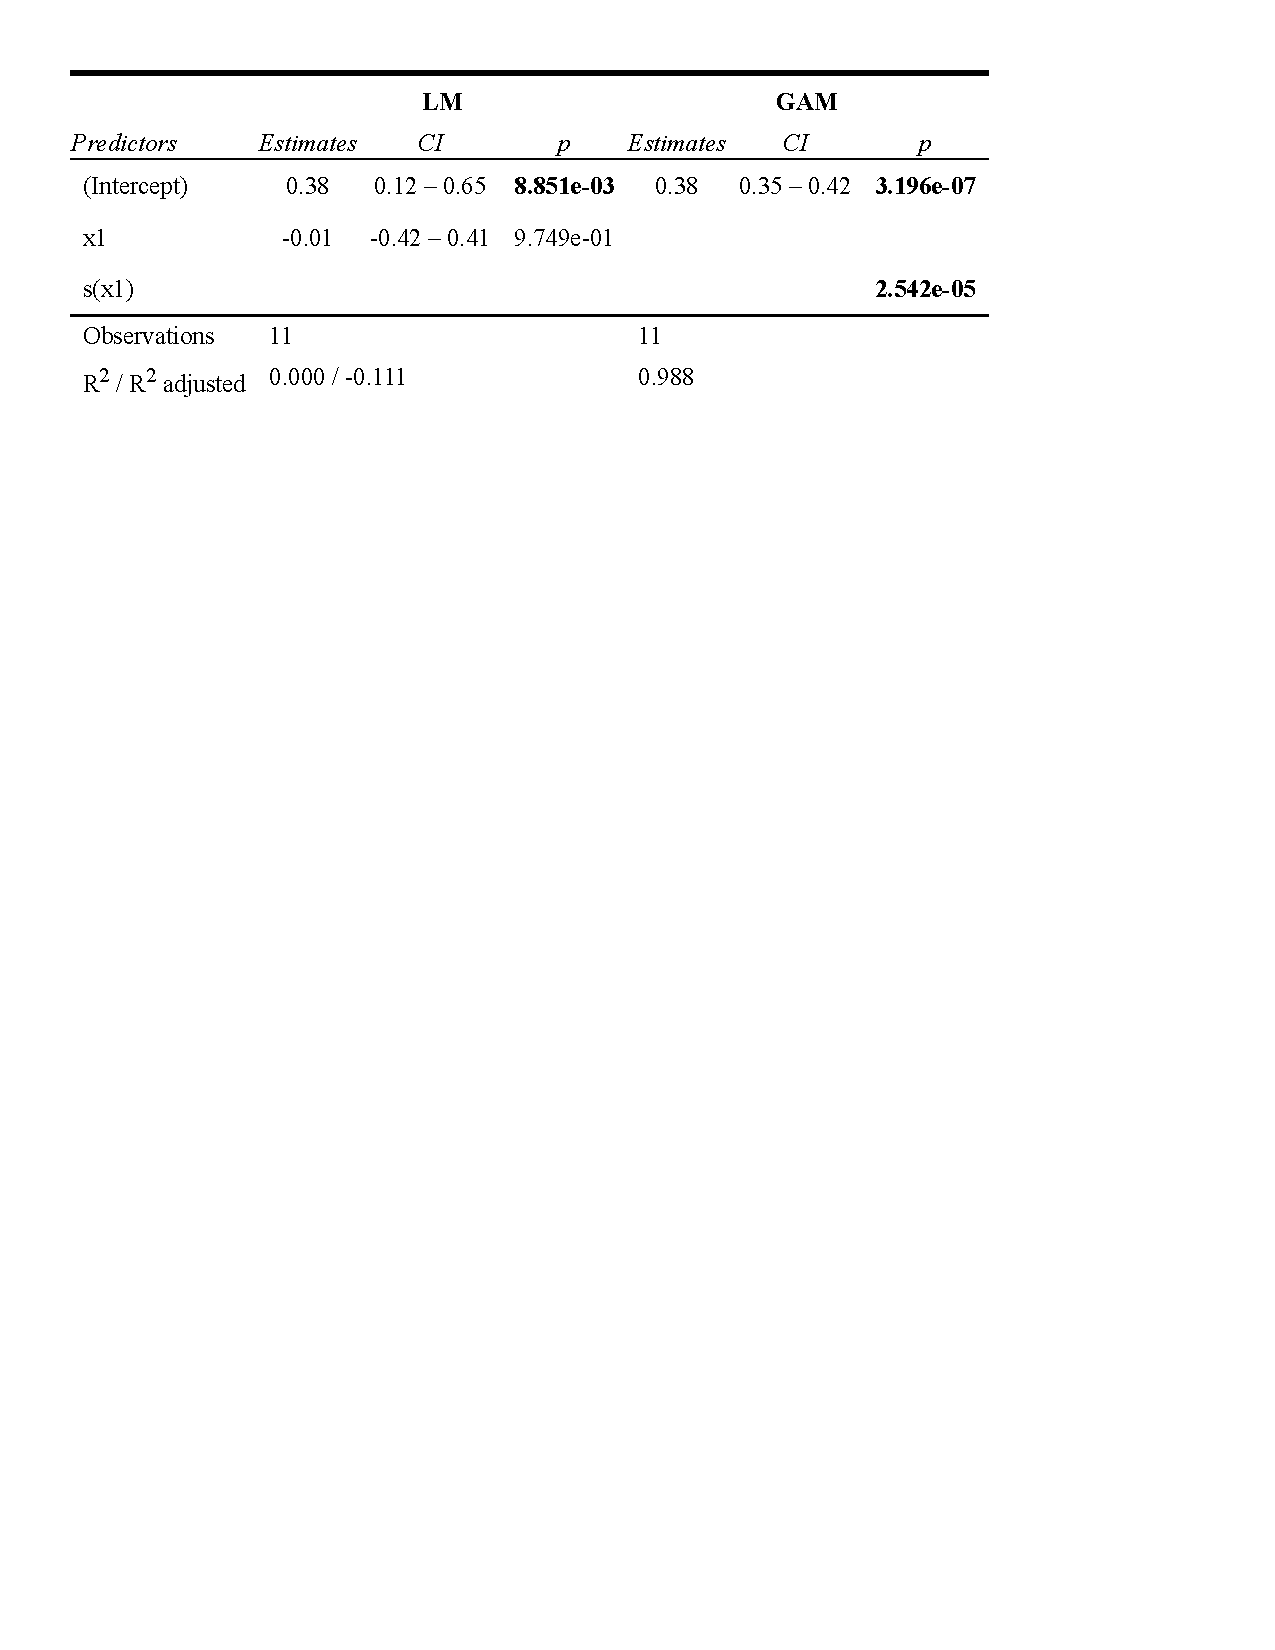
\includegraphics[clip, trim=0.5cm 21cm 5cm 1cm, width=.6\textwidth]{figure/GAM_LM_Output.pdf}
\end{center}
The R$^2-$value for the GAM model is the adjusted one.

\bigskip

What is the \textbf{Adjusted R}$\bold{^2}$? 

Problem with $R^2$:  $R^2$ rises each time a feature is added, no matter if the added feature improves the fit or not.

The adjusted $R^2$ considers the number of terms in a model and only increases after adding a feature, if the fit becomes better:
$$ \text{adj. } R^2 = 1-\frac{SSE_{LM}\, / \, (n-p-1)}{SSE_{c}\, / \, (n-1)}, $$
where $n$ is the sample size and $p$ is the number of features.

Hence, it is the proportion of explained variance using unbiased estimates.

\begin{enumerate}[a)]
	\item LM: Since the $\beta$-values are not scaled, they are not well interpretable. From the high p-value and $R^2$ = 0 it can be inferred that there is no linear relationship. (Remember: $R^2 = \rho^2$. )
	\item GAM: The p-value of $2.54 \times 10^{-5}$ (but also the adjusted $R^2$ value) reveals that there is a strong relationship between $x_1$ and $x_2$. Hence, generalized additive models (GAM) are able to detect non-linear relationships. The p-value does not reveal the shape of this relationship. 
	\begin{center}
		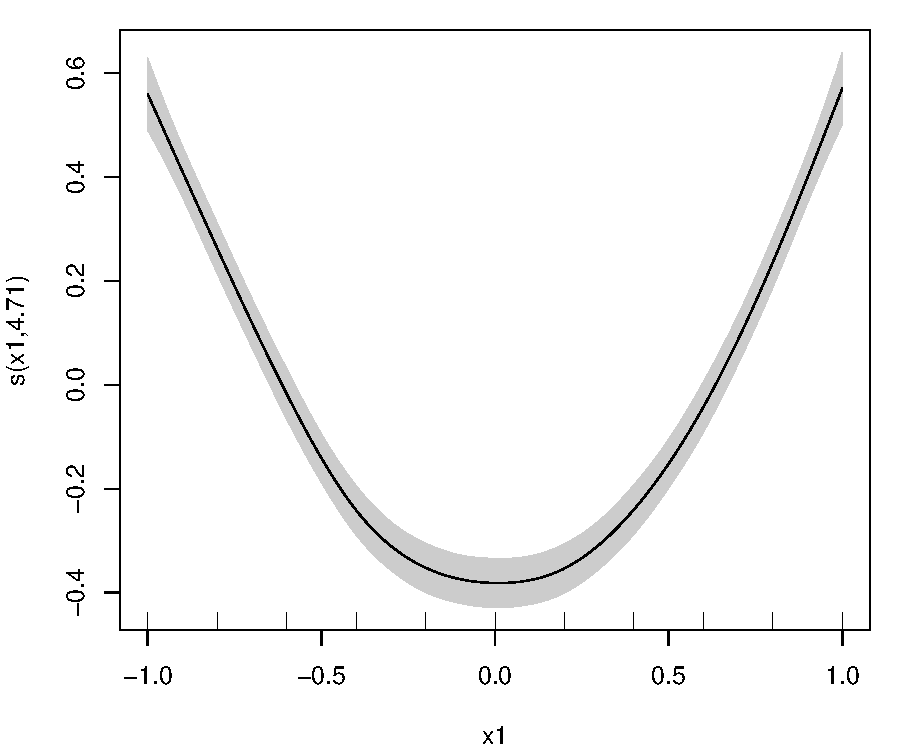
\includegraphics[width=.6\textwidth]{figure/gam.pdf}
	\end{center}
\end{enumerate}

}
